\documentclass[11pt,aspectratio=169]{beamer}

% --- Theme & look ---
\usetheme{Madrid}
\setbeamertemplate{navigation symbols}{}
\setbeamertemplate{blocks}[rounded][shadow=false]
\useinnertheme{rounded}
\usefonttheme{professionalfonts}

% Slightly larger, more readable beamer typography
\setbeamerfont{frametitle}{size=\Large}
\setbeamerfont{block title}{size=\large}
\setbeamerfont{block title alerted}{size=\large}

% --- Language & fonts (XeLaTeX + Babel) ---
\usepackage{fontspec}
\usepackage[main=greek,english]{babel}

% Fonts with Greek support (shipped with TeX distributions)
\defaultfontfeatures{Ligatures=TeX}
% Use common Windows fonts to avoid font lookup issues
\setsansfont{Calibri}
\setmainfont{Cambria}
\setmonofont{Consolas}

\usepackage{microtype}

% --- Utilities ---
\usepackage{booktabs}
\usepackage{graphicx}
\usepackage{ragged2e}
\usepackage{hyperref}
\usepackage{tikz}
\usetikzlibrary{arrows.meta,positioning,calc,fit,shapes.geometric}

% --- Custom commands (Greek text + English terms) ---
\newcommand{\latin}[1]{\foreignlanguage{english}{#1}}
\newcommand{\eng}[1]{\foreignlanguage{english}{#1}}
\newcommand{\term}[2]{#1 (\eng{#2})}
\newcommand{\code}[1]{\texttt{\foreignlanguage{english}{#1}}}
\newcommand{\smallcode}[1]{{\footnotesize\texttt{\foreignlanguage{english}{#1}}}}
\newcommand{\sigil}[1]{\foreignlanguage{english}{\texttt{\textbf{#1}}}}
\newcommand{\krrsep}{\hspace{0.8em}\textcolor{black!40}{\(\cdot\)}\hspace{0.8em}}
\newcommand{\aspcode}[1]{\foreignlanguage{english}{{\footnotesize\nolinkurl{#1}}}}

% --- Colors (single blue system) ---
\definecolor{KRRBlue}{RGB}{13,71,161}
\definecolor{KRRGray}{RGB}{38,50,56}
\setbeamercolor{title}{fg=white,bg=KRRBlue}
\setbeamercolor{frametitle}{fg=white,bg=KRRBlue}
\setbeamercolor{structure}{fg=KRRBlue}
\setbeamercolor{block title}{fg=white,bg=KRRBlue}
\setbeamercolor{block body}{bg=black!2}
\setbeamercolor{block title alerted}{fg=white,bg=KRRBlue}
\setbeamercolor{block body alerted}{bg=black!2}
\setbeamercolor{block title example}{fg=white,bg=KRRBlue}
\setbeamercolor{block body example}{bg=black!2}
\setbeamercolor{alerted text}{fg=KRRBlue}

% --- Footline (clean + slide numbers) ---
\setbeamertemplate{footline}{
  \leavevmode%
  \hbox{%
    \begin{beamercolorbox}[wd=.85\paperwidth,ht=2.6ex,dp=1.2ex,leftskip=0.8em]{author in head/foot}%
      \usebeamerfont{author in head/foot}\insertshorttitle\krrsep\insertshortinstitute
    \end{beamercolorbox}%
    \begin{beamercolorbox}[wd=.15\paperwidth,ht=2.6ex,dp=1.2ex,center]{date in head/foot}%
      \usebeamerfont{date in head/foot}\insertframenumber/\inserttotalframenumber
    \end{beamercolorbox}%
  }%
}

% (No section-only title frames.)

% --- Title info ---
\title[\eng{ASP} \& \eng{Spack}]{\eng{Answer Set Programming for HPC Dependency Solving}}
\author[\eng{KRR}]{Κωνσταντίνος Καϊμάκης (mtn2508)\\Γιώργος Νάζος (mtn2519) \quad Γιώργος Πλέσσιας (mtn2524) \quad Ορέστης Τσαγκέτας (mtn2527)}
\date{12 Φεβρουαρίου 2026}

\begin{document}

% --- Title ---
\begin{frame}[plain]
  \vspace*{0.2cm}
  \begin{center}
    {\color{KRRBlue}\LARGE\bfseries \inserttitle \par}
    \vspace{0.30cm}
    
\begin{tikzpicture}
      \draw[KRRBlue, line width=1.6pt] (0,0) -- (11.0,0);
    \end{tikzpicture}
  \end{center}

  \vfill
  \begin{center}
    {\footnotesize \insertauthor \par}
    \vspace{0.1cm}
    {\footnotesize \insertinstitute \par}
  \end{center}
  \vfill
  \begin{center}
    {\footnotesize \insertdate \par}
  \end{center}
\end{frame}

% --- Agenda ---
\begin{frame}{Δομή}
  \begin{itemize}
    \item Γιατί το \eng{HPC} κάνει το πρόβλημα δύσκολο
    \item \eng{Spack specs} και \eng{concretization}
    \item Μοντελοποίηση σε \eng{ASP}: facts / rules / constraints
    \item \eng{Virtual dependencies}, \eng{conditional dependencies}, \eng{variants}
    \item Βελτιστοποίηση + \eng{reuse}
    \item Αποτελέσματα / περιορισμοί
  \end{itemize}
\end{frame}

\section{Το πρόβλημα στο \eng{HPC}}

\begin{frame}{ \eng{HPC dependency resolution}}
  \begin{columns}[T,onlytextwidth]
    \begin{column}{0.56\textwidth}
      \begin{block}{\eng{HPC Stack}}
        \begin{itemize}
          \item \textbf{Εκδόσεις}: πολλαπλές εκδόσεις συνυπάρχουν
          \item \textbf{Compilers}: \eng{GCC} \(\Rightarrow\) \eng{ABI} ασυμβατότητες
          \item \textbf{Variants}: \code{+mpi}, \code{+cuda}, \code{\textasciitilde{}debug}, \dots
          \item \textbf{Targets}: \eng{Skylake}/\eng{Power9}/\eng{GPU}, \dots
        \end{itemize}
      \end{block}
      \vspace{0.2cm}
      \begin{alertblock}{Το πρόβλημα}
        \justifying
        Ο γράφος είναι \eng{DAG}, αλλά κάθε κόμβος είναι \textbf{package} και τα \textbf{edges} είναι \textbf{dependencies}.
        Το γενικό πρόβλημα είναι \textbf{\eng{NP-complete}}.
      \end{alertblock}
    \end{column}
    \begin{column}{0.40\textwidth}
      \begin{block}{Διαισθητικό διάγραμμα}
        \centering
        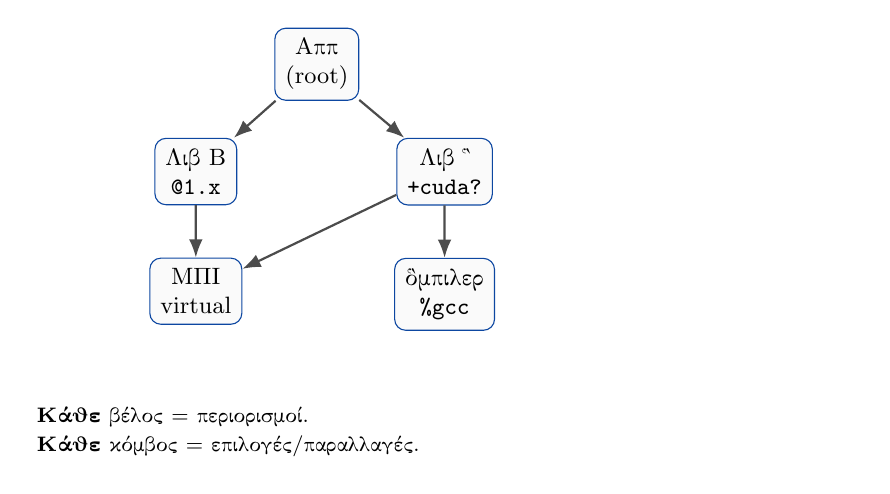
\begin{tikzpicture}[node distance=7mm, font=\small, scale=0.95, transform shape]
          \tikzset{
            pkg/.style={rounded corners, draw=KRRBlue, fill=black!2, inner sep=4pt, align=center},
            dep/.style={-Latex, thick, draw=black!70}
          }
          \node[pkg] (A) {App\\\eng{(root)}};
          \node[pkg, below left=of A] (B) {Lib B\\\code{@1.x}};
          \node[pkg, below right=of A] (C) {Lib C\\\code{+cuda?}};
          \node[pkg, below=of B] (D) {MPI\\\eng{virtual}};
          \node[pkg, below=of C] (E) {Compiler\\\code{\%gcc}};
          \draw[dep] (A) -- (B);
          \draw[dep] (A) -- (C);
          \draw[dep] (B) -- (D);
          \draw[dep] (C) -- (D);
          \draw[dep] (C) -- (E);
          \node[align=left, text width=0.90\linewidth, below=9mm of E] {\footnotesize
            \textbf{Κάθε} βέλος = περιορισμοί.\\
            \textbf{Κάθε} κόμβος = επιλογές/παραλλαγές.
          };
        \end{tikzpicture}
      \end{block}
    \end{column}
  \end{columns}
\end{frame}

\begin{frame}{ Υπάρχοντες \eng{HPC package managers}}
  \begin{columns}[T,onlytextwidth]
    \begin{column}{0.48\textwidth}
      \begin{block}{\eng{System package managers} (\eng{APT}/\eng{RPM})}
        \begin{itemize}
          \item κοινό \eng{prefix} (\eng{/usr}) \(\Rightarrow\) 1 έκδοση/πακέτο
          \item πιο «στενός» χώρος αναζήτησης από \eng{HPC}
        \end{itemize}
      \end{block}
      \begin{block}{\eng{Language managers} (\eng{pip}/\eng{cargo})}
        \begin{itemize}
          \item συχνά αγνοούν system deps (\eng{C/C++}, compilers)
          \item \eng{ad-hoc} επίλυση
        \end{itemize}
      \end{block}
    \end{column}
    \begin{column}{0.48\textwidth}
      \begin{alertblock}{Το παλιό \eng{Spack} (\eng{greedy})}
        \begin{itemize}
          \item αποφάσεις «χωρίς επιστροφή» (\eng{no backtracking})
          \item \textbf{false negatives}: αποτυγχάνει ενώ υπάρχει λύση
        \end{itemize}
      \end{alertblock}
      \vspace{0.2cm}
      \begin{block}{Τι θέλουμε}
        \begin{itemize}
          \item \textbf{Πληρότητα}: αν υπάρχει λύση, να βρεθεί
          \item \textbf{Βελτιστότητα}: εύρεση βέλτιστης λύσης
          \item \textbf{Συντηρησιμότητα}: κανόνες, όχι \eng{complex} \eng{heuristics}
        \end{itemize}
      \end{block}
    \end{column}
  \end{columns}
\end{frame}

\section{Από \eng{Spec} σε \eng{DAG}: ο \eng{concretizer}}

\begin{frame}{\eng{Spack spec syntax}}
  \begin{block}{Περιορισμοί}
    \begin{itemize}
      \item \sigil{@} έκδοση: \code{hdf5@1.10.2}
      \item \sigil{\%} μεταγλωττιστής: \code{\%gcc@9.3.0}
      \item \sigil{+}/\sigil{\textasciitilde{}} variants: \code{+mpi}, \code{\textasciitilde{}shared}
      \item \sigil{\string^} εξάρτηση: \code{\string^mpich@3.3}
    \end{itemize}
  \end{block}

  \begin{alertblock}{Παράδειγμα}
    \smallcode{spack install hdf5@1.10.2+mpi \%gcc@9.3.0 \string^mpich@3.3}
  \end{alertblock}

  \begin{block}{\eng{Concretization}}
    \justifying
    Συμπληρώνοντας τα κενά με \eng{constraints} έτσι ώστε:
    (i) να ικανοποιούνται περιορισμοί χρήστη/πακέτων/περιβάλλοντος, και (ii) να μην υπάρχουν \eng{conflicts}.
  \end{block}
\end{frame}

\section{\eng{ASP}: Facts, Rules, Constraints}

\begin{frame}{\eng{ASP Implementation}}
  \begin{columns}[T,onlytextwidth]
    \begin{column}{0.54\textwidth}
      \begin{block}{\eng{Declarative} μοντέλο}
        \begin{itemize}
          \item \textbf{Facts}: δεδομένα (\eng{available versions}, deps)
          \item \textbf{Rules}: παραγωγή γνώσης (\eng{propagation})
          \item \textbf{Constraints}: τι απαγορεύεται
        \end{itemize}
      \end{block}
      \begin{block}{Ροή}
        \begin{itemize}
          \item \textbf{Python} παράγει facts
          \item \textbf{Grounding} \(\rightarrow\) προτασιακό πρόγραμμα
          \item \textbf{\eng{clingo}} \(\rightarrow\) \term{stable models}{stable models}
        \end{itemize}
      \end{block}
    \end{column}
    \begin{column}{0.44\textwidth}
      \begin{block}{Παράδειγμα pipeline}
        \centering
        \resizebox{0.98\linewidth}{!}{%
          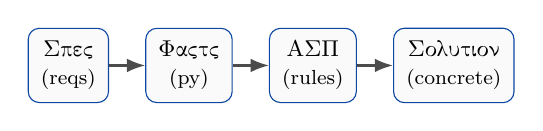
\begin{tikzpicture}[font=\small, node distance=5mm, scale=0.92, transform shape]
            \tikzset{
              box/.style={rounded corners, draw=KRRBlue, fill=black!2, inner sep=5pt, align=center},
              arr/.style={-Latex, thick, draw=black!70}
            }
            \node[box] (spec) {Spec\\\footnotesize(\eng{reqs})};
            \node[box, right=of spec] (facts) {Facts\\\footnotesize(\eng{py})};
            \node[box, right=of facts] (asp) {ASP\\\footnotesize(\eng{rules})};
            \node[box, right=of asp] (sol) {Solution\\\footnotesize(\eng{concrete})};
            \draw[arr] (spec) -- (facts);
            \draw[arr] (facts) -- (asp);
            \draw[arr] (asp) -- (sol);
          \end{tikzpicture}%
        }
      \end{block}
      \begin{alertblock}{Γιατί όχι καθαρό \eng{SAT};}
        \justifying
        Το μοντέλο \eng{HPC} είναι εκφραστικά «βαρύ». Ο \eng{ASP} δίνει πιο φυσικούς/συντηρήσιμους κανόνες.
      \end{alertblock}
    \end{column}
  \end{columns}
\end{frame}

\begin{frame}{Παράδειγμα}
  \begin{block}{Πακέτα, εκδόσεις, deps}
    \justifying
    Η Python μεταφράζει τη γνώση των \code{package.py} σε facts, π.χ.:
    \vspace{0.2cm}

    \begin{center}
      \fbox{\parbox{0.92\linewidth}{
        \small
        \eng{package("zlib").}\\
        \eng{version\_declared("zlib","1.2.11",0).}\\
        \eng{possible\_dependency("hdf5","mpi").}
      }}
    \end{center}
  \end{block}
  \begin{alertblock}{Σχόλιο}
    \justifying
    Για ένα ρεαλιστικό πρόβλημα δημιουργούνται \textbf{δεκάδες χιλιάδες} facts πριν καν ξεκινήσει το solving.
  \end{alertblock}
\end{frame}

\begin{frame}{Κανόνας επιλογής: «μία έκδοση ανά κόμβο»}
  \begin{block}{Choice rule (πυρήνας)}
    \begin{center}
      \fbox{\parbox{0.92\linewidth}{
        \small
        \aspcode{1 \{ version(P,V) : possible_version(P,V) \} 1 :- node(P).}
      }}
    \end{center}
  \end{block}
  \begin{columns}[T,onlytextwidth]
    \begin{column}{0.54\textwidth}
      \begin{block}{Τι σημαίνει}
        \begin{itemize}
          \item για κάθε \eng{node(P)} επιλέγουμε \textbf{ακριβώς 1} \eng{V}
          \item αποκλείει «διπλές» εκδόσεις στον ίδιο κόμβο λύσης
        \end{itemize}
      \end{block}
    \end{column}
    \begin{column}{0.44\textwidth}
      \begin{alertblock}{Σύγκριση}
        \justifying
        Αντί για διαδικαστικό backtracking, το backtracking γίνεται \textbf{εσωτερικά} στον solver.
      \end{alertblock}
    \end{column}
  \end{columns}
\end{frame}

\begin{frame}{Διάδοση εξαρτήσεων: «αν υπάρχει πακέτο, υπάρχουν και οι deps»}
  \begin{block}{Propagation rule}
    \begin{center}
      \fbox{\parbox{0.92\linewidth}{
        \small
        \aspcode{node(Dep) :- node(Pkg), depends_on(Pkg,Dep).}
      }}
    \end{center}
  \end{block}
  \begin{columns}[T,onlytextwidth]
    \begin{column}{0.54\textwidth}
      \begin{block}{Κέρδος}
        \justifying
        Ο γράφος «χτίζεται» λογικά και ο solver εξερευνά ταυτόχρονα τις επιλογές σε βάθος, χωρίς να εγκλωβίζεται
        από πρώιμες επιλογές.
      \end{block}
    \end{column}
    \begin{column}{0.44\textwidth}
      \begin{alertblock}{Στην πράξη}
        \justifying
        Αυτό είναι η βάση για \textbf{πληρότητα}: αν υπάρχει λύση, θα βρεθεί.
      \end{alertblock}
    \end{column}
  \end{columns}
\end{frame}

\section{\eng{Virtuals}, \eng{Conditionals}, \eng{Variants}}

\begin{frame}{\term{Virtual dependencies}{virtuals}: επιλογή παρόχου}
  \begin{columns}[T,onlytextwidth]
    \begin{column}{0.56\textwidth}
      \begin{block}{Ιδέα}
        \justifying
        Για δυνατότητες τύπου \eng{MPI}, δεν ζητάμε «πακέτο», ζητάμε \textbf{λειτουργία}. Ο solver επιλέγει provider.
      \end{block}
      \begin{block}{Κανόνας (σχηματικά)}
        \begin{center}
          \fbox{\parbox{0.92\linewidth}{
            \small
            \aspcode{1 \{ provider(V, P) : provides(P, V) \} 1 :- node(P), depends_on(P, V).}
            % \aspcode{1 \{ provider(Virt,Pkg) : provides(Pkg,Virt) \} 1 :- node(P), depends_on(P,Virt).}
          }}
        \end{center}
      \end{block}
    \end{column}
    \begin{column}{0.40\textwidth}
      \begin{block}{Παράδειγμα}
        \begin{itemize}
          \item \eng{hdf5} depends on \eng{mpi}
          \item providers: \eng{mpich}, \eng{openmpi}
          \item επιλογή βάσει \term{preferences}{preferences} + συγκρούσεων
        \end{itemize}
      \end{block}
      \begin{alertblock}{Σημείο-κλειδί}
        \justifying
        Η επιλογή provider είναι μέρος της ίδιας ενιαίας βελτιστοποίησης.
      \end{alertblock}
    \end{column}
  \end{columns}
\end{frame}

\begin{frame}{\term{Conditional deps}{conditionals}: όταν μια εξάρτηση εξαρτάται από variant}
  \begin{columns}[T,onlytextwidth]
    \begin{column}{0.54\textwidth}
      \begin{block}{Πρόβλημα (greedy)}
        \justifying
        Πρέπει να «μαντέψεις» πρώτα το \code{+bzip2} ή όχι, αλλιώς μπορεί να πέσεις σε αδιέξοδο.
      \end{block}
      \begin{block}{ASP (γενικευμένες συνθήκες)}
        \justifying
        Ο solver αποφασίζει \textbf{ταυτόχρονα} τις τιμές των \eng{variants} και το αν ενεργοποιείται η αντίστοιχη εξάρτηση.
        \vspace{0.2cm}

        \begin{center}
          \fbox{\parbox{0.92\linewidth}{
            \small
            \aspcode{condition_holds(ID) :- node(P), variant_value(P,bzip2,true). dependency_enabled(P,bzip2) :- condition_holds(ID).}
          }}
        \end{center}
      \end{block}
    \end{column}
    \begin{column}{0.42\textwidth}
      \begin{alertblock}{Γιατί είναι δυνατό}
        \justifying
        O solver εξετάζει όλο τον χώρο αναζήτησης και κάνει backtracking όπου χρειαστεί.
      \end{alertblock}
      \begin{block}{Αποτέλεσμα}
        \begin{itemize}
          \item λιγότερα αδιέξοδα
          \item πιο «σωστές» λύσεις σε σύνθετα specs
        \end{itemize}
      \end{block}
    \end{column}
  \end{columns}
\end{frame}

\section{Βελτιστοποίηση: από έγκυρο σε βέλτιστο}

\begin{frame}{Λεξικογραφική πολυκριτηριακή βελτιστοποίηση}
  \begin{columns}[T,onlytextwidth]
    \begin{column}{0.60\textwidth}
      \begin{block}{Ιδέα}
        \justifying
        Δεν αρκεί «να υπάρχει λύση». Θέλουμε λύση που να ακολουθεί ιεραρχημένες προτιμήσεις (lexicographic).
      \end{block}
      \begin{block}{Ενδεικτικά κριτήρια (υψηλή προτεραιότητα)}
        \begin{itemize}
          \item \textbf{Deprecated versions}: αποφυγή μη ασφαλών/παρωχημένων
          \item \textbf{Version age (roots)}: νεότερες εκδόσεις για roots
          \item \textbf{Variant defaults (roots)}: τήρηση defaults όπου γίνεται
          \item \textbf{Preferred providers}: π.χ. \eng{MPICH} αντί \eng{OpenMPI}
        \end{itemize}
      \end{block}
    \end{column}
    \begin{column}{0.36\textwidth}
      \begin{alertblock}{Συνέπεια}
        \justifying
        Κριτήριο 1 υπερισχύει απόλυτα του 2: \textbf{κανένα trade-off} που «σπάει» την ασφάλεια.
      \end{alertblock}
      \begin{block}{Συνοχή στο \eng{HPC}}
        \begin{itemize}
          \item \textbf{Compiler mismatch} \(\downarrow\) (ABI)
          \item \textbf{Target mismatch} \(\downarrow\)
        \end{itemize}
      \end{block}
    \end{column}
  \end{columns}
\end{frame}

\begin{frame}{Καινοτομία: \term{software reuse}{reuse} + \term{buildcache}{buildcache}}
  \begin{columns}[T,onlytextwidth]
    \begin{column}{0.56\textwidth}
      \begin{block}{Το «κόλπο» με τους κάδους}
        \justifying
        Διπλασιάζουμε κριτήρια: άλλα για \textbf{νέα builds} και άλλα για \textbf{εγκατεστημένα} (reused) πακέτα,
        και εισάγουμε ενδιάμεσα στόχο: \textbf{ελαχιστοποίηση builds}.
      \end{block}
      \begin{alertblock}{Λογική πολιτική}
        \justifying
        «Αν πρέπει να χτίσεις, χτίσε το τέλειο. Αν υπάρχει συμβατό binary, προτίμησέ το για να γλιτώσεις χρόνο».
      \end{alertblock}
    \end{column}
    \begin{column}{0.40\textwidth}
      \begin{block}{Γιατί έχει σημασία}
        \small
        \begin{itemize}
          \item builds στο \eng{HPC} είναι ακριβά (χρόνος/πόροι)
          \item reuse = γρηγορότερα installs \(\Rightarrow\) καλύτερο UX
        \end{itemize}
      \end{block}
      \begin{block}{Σχηματικό}
        \centering
        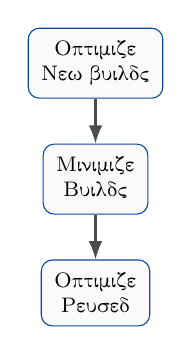
\begin{tikzpicture}[font=\footnotesize, scale=0.95, transform shape]
          \tikzset{
            b/.style={rounded corners, draw=KRRBlue, fill=black!2, inner sep=5pt, align=center},
            arr/.style={-Latex, thick, draw=black!70}
          }
          \node[b] (new) {Optimize\\New builds};
          \node[b, below=6mm of new] (min) {Minimize\\Builds};
          \node[b, below=6mm of min] (old) {Optimize\\Reused};
          \draw[arr] (new) -- (min);
          \draw[arr] (min) -- (old);
        \end{tikzpicture}
      \end{block}
    \end{column}
  \end{columns}
\end{frame}

\section{Αποτελέσματα \& περιορισμοί}

\begin{frame}{Απόδοση στην πράξη (\eng{E4S} και πραγματικά \eng{HPC} συστήματα)}
  \begin{columns}[T,onlytextwidth]
    \begin{column}{0.54\textwidth}
      \begin{block}{Περιβάλλον}
        \begin{itemize}
          \item \eng{E4S} repository (χιλιάδες πακέτα)
          \item \eng{Quartz} (\eng{Intel Xeon}) και \eng{Lassen} (\eng{Power9 + NVIDIA GPU})
        \end{itemize}
      \end{block}
      \begin{block}{Κύρια ευρήματα}
        \begin{itemize}
          \item \textbf{Solve times}: συνήθως \(\mathbf{< 1}\) sec
          \item χρόνος \(\uparrow\) με πολλές \term{εναλλακτικές εξαρτήσεις}{choices}
          \item ρύθμιση \eng{clingo} \textbf{tweety} καλύτερη (έναντι \eng{trendy}/\eng{handy})
        \end{itemize}
      \end{block}
    \end{column}
    \begin{column}{0.44\textwidth}
      \begin{alertblock}{Κλιμάκωση με reuse}
        \justifying
        Ακόμη και με \(\sim\)63.099 εγκατεστημένα πακέτα (buildcache), ο solver παραμένει γρήγορος.
      \end{alertblock}
      \begin{block}{Πού είναι το bottleneck;}
        \justifying
        Μετατοπίζεται στην \textbf{\eng{Python setup phase}} (εξαγωγή facts/grounding),
        όχι στο ίδιο το solving.
      \end{block}
    \end{column}
  \end{columns}
\end{frame}

\begin{frame}{Ποιότητα λύσεων: το τέλος των \eng{false negatives}}
  \begin{columns}[T,onlytextwidth]
    \begin{column}{0.58\textwidth}
      \begin{block}{Τι άλλαξε ουσιαστικά}
        \begin{itemize}
          \item επιλύει σενάρια όπου ο greedy αποτυγχάνει
          \item καλύτερος χειρισμός: συγκρούσεις εκδόσεων + conditionals
          \item λύσεις \textbf{εγγυημένα βέλτιστες} βάσει κριτηρίων
        \end{itemize}
      \end{block}
      \begin{alertblock}{Συντηρησιμότητα}
        \justifying
        Κανόνες ASP \(\approx\) «γνώση» του συστήματος. Πιο καθαρό από heuristics που ξεφεύγουν με τον χρόνο.
      \end{alertblock}
    \end{column}
    \begin{column}{0.40\textwidth}
      \begin{block}{Σύνοψη σύγκρισης}
        \footnotesize
        \begin{tabular}{@{}p{0.55\linewidth}p{0.38\linewidth}@{}}
          \toprule
          \textbf{Χαρακτηριστικό} & \textbf{ASP concretizer} \\
          \midrule
          Πληρότητα & Ναι \\
          Βελτιστοποίηση & Πολυκριτηριακή \\
          Variants/Conditionals & Φυσικά ενσωματωμένα \\
          Συντηρησιμότητα & Υψηλή \\
          \bottomrule
        \end{tabular}
      \end{block}
    \end{column}
  \end{columns}
\end{frame}

\begin{frame}{Περιορισμοί / τι μένει δύσκολο}
  \begin{columns}[T,onlytextwidth]
    \begin{column}{0.50\textwidth}
      \begin{alertblock}{Setup overhead}
        \justifying
        Η γείωση + παραγωγή facts (Python) μπορεί να καθυστερήσει απλές εντολές.
      \end{alertblock}
      \begin{block}{Debugging όταν δεν υπάρχει λύση}
        \justifying
        \eng{SAT}-style εξηγήσεις (\eng{unsat cores}) δεν είναι πάντα «φιλικές» στον χρήστη.
      \end{block}
    \end{column}
    \begin{column}{0.46\textwidth}
      \begin{block}{Προοπτικές}
        \begin{itemize}
          \item βελτιστοποίηση setup phase (Python)
          \item \term{incremental solving}{incremental solving}
          \item εφαρμογή ιδέας σε \eng{cloud orchestration}/\eng{microservices}
        \end{itemize}
      \end{block}
      \begin{block}{Takeaway (1 πρόταση)}
        \justifying
        \textbf{Ο ASP μετατρέπει την επίλυση εξαρτήσεων από ευριστικό «κόλπο» σε μαθηματικά ελεγχόμενη διαδικασία.}
      \end{block}
    \end{column}
  \end{columns}
\end{frame}

\section{Κλείσιμο}

\begin{frame}{Συμπέρασμα (για \eng{KRR})}
  \begin{block}{Πού «κουμπώνει» στο μάθημα;}
    \begin{itemize}
      \item Αναπαράσταση γνώσης: facts/rules/constraints ως μοντέλο του οικοσυστήματος πακέτων
      \item Αυτόματη συλλογιστική: stable models ως λύσεις του concretization
      \item Βελτιστοποίηση: τυπικά κριτήρια, όχι ad-hoc heuristics
    \end{itemize}
  \end{block}
  \begin{alertblock}{Μήνυμα}
    \justifying
    Όταν το πρόβλημα είναι συνδυαστικό και γεμάτο περιορισμούς, το \textbf{να το γράψεις ως λογική} μπορεί να είναι
    πιο πρακτικό από το να «μπαλώσεις» heuristics.
  \end{alertblock}
\end{frame}

\begin{frame}[plain]
  \vfill
  \begin{center}
    {\Huge\color{KRRBlue} Ευχαριστούμε για την προσοχή σας!}\\[0.4cm]
    \vspace{0.8cm}

    {\footnotesize \textcolor{black!45}{Πηγή: \eng{Gamblin et al. (2022)} — \code{paper.pdf} (με highlights σε σελ. 4–12)}}
  \end{center}
  \vfill
\end{frame}

\end{document}

